\documentclass{article}
% preámbulo

\usepackage[utf8]{inputenc} % Para escribir tildes
\usepackage[T1]{fontenc}    % Para usar fuentes con letras acentuadas, etc.
\usepackage[spanish]{babel} % Definimos el idioma principal
\usepackage{graphicx} %Para las imagenes

\title{Analizador Léxico y Tabla de Símbolos}
\author{Aarón Cabero Blanco \\ Daniel Tomás Sanchez \\ Alejandro Cuadrón Lafuente}

\begin{document}

\maketitle
En este documento se realizará la memoria del analizador léxico y la tabla de símbolos correspondiente a la primera entrega de la practica de PDL.
\clearpage%para saltar a otra página
%dividimos en secciones


\section {Tokens}
\begin{flushleft}
\begin{itemize}
\item Identificador \qquad\qquad<ID, punteroTS>
\item Constante Entera \qquad\qquad<CTEENTERA, valor>
\item String \qquad\qquad<CADENA, lexema>	
\item False \qquad\qquad<CTELOGICA, 0> 
\item True \qquad\qquad<CTELOGICA, 1> 
\item Palabra Reservada Number\qquad\qquad<NUMBER, ->
\item Palabra Reservada String\qquad\qquad<STRING, ->
\item Palabra Reservada Boolean\qquad\qquad<BOOLEAN, ->
\item Palabra Reservada Let\qquad\qquad<LET, ->
\item Palabra Reservada Alert\qquad\qquad<ALERT, ->
\item Palabra Reservada Input\qquad\qquad<INPUT, ->
\item Palabra Reservada Function\qquad\qquad<FUNCTION, ->
\item Palabra Reservada Return \qquad\qquad<RETURN, ->
\item Palabra Reservada If \qquad\qquad<IF, ->
\item Palabra Reservada For\qquad\qquad<FOR, ->
\item -- \qquad\qquad<OPESP, -> 
\item + \qquad\qquad<OPARIT, 0> 
\item -  \qquad\qquad<OPARIT, 1>
\item =\qquad\qquad <OPASIGN, -> 
\item == \qquad\qquad<OPREL, ->
\item \&\& \qquad\qquad<OPLOG, -> 
\item ( \qquad\qquad<ABREPAR, ->
\item ) \qquad\qquad<CIERRAPAR,> 
\item \{ \qquad\qquad<ABRELLAVE, ->
\item \} \qquad\qquad<CIERRALLAVE, ->
\item , \qquad\qquad<COMA, ->
\item ; \qquad\qquad<PUNTOYCOMA, ->
\item End Of File \qquad\qquad<EOF, ->

\end{itemize}
\end{flushleft}
\clearpage


\section{Gramática Regular}
\noindent
Axioma = A\\
A $\rightarrow$ del A $|$ dD $|$ "S $|$ /C $|$ lI $|$ + $|$ -M $|$ =E $|$ \&N $|$ ( $|$ ) $|$ \{ $|$ \} $|$ ; $|$ , $|$ EOF\\
D $\rightarrow$ dD $|$ $\lambda$\\
S $\rightarrow$ " $|$ cS\\
C $\rightarrow$ *C'\\
C' $\rightarrow$ *C'' $|$ cC'\\
C'' $\rightarrow$ /A $|$ cC'\\
I $\rightarrow$ dI $|$ lI $|$ \_I $|$ $\lambda$\\
M $\rightarrow$ - $|$ $\lambda$\\
E $\rightarrow$ = $|$ $\lambda$\\
N $\rightarrow$ \&\\
\\
Siendo $d$ un dígito, $l$ una letra, $c$ cualquier otro carácter y $del$ un delimitador.
\section{Autómata Finito Determinista}
\begin{center}
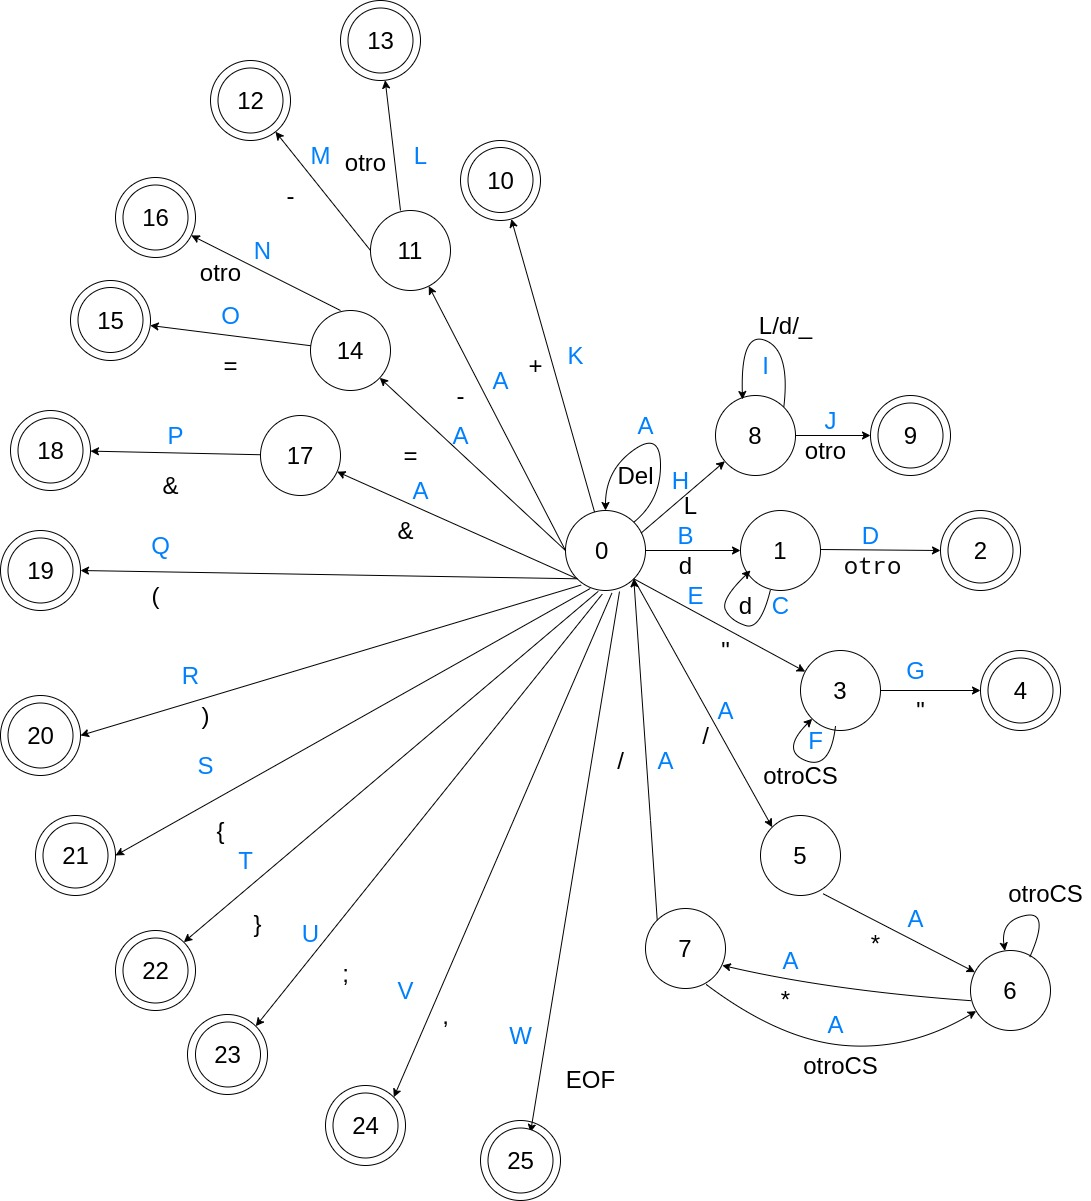
\includegraphics[scale=0.26]{automata.jpg}
\end{center}


\section{Acciones Semánticas}
\begin{flushleft}
A: leer\\
B: number = int(d), leer\\
C: number = number*10 + int(d), leer\\
D: if number>32767\\
       \qquad pError("Número fuera de rango")\\
   \quad else \\
        \qquad genToken(CTEENTERA,number);\\
E: string = '', contador = 0, leer\\
F: string = string + otroCS, contador++ leer\\
G: if contador>64\\
       \qquad pError("Cadena demasiado larga")\\
   \quad else\\
        \qquad genToken(CADENA,string)\\
  \quad leer\\
H: string = l, leer\\
I: string = string + l/D/\_ , leer\\
J: if palabrasReservadas.contains(string)\\
       \qquad if string == "number"\\
      \qquad \quad      genToken(NUMBER,-)\\
       \qquad elif string == "string"\\
       \qquad \quad     genToken(STRING,-)\\
      \qquad  elif string == "boolean"\\
      \qquad \quad      genToken(BOOLEAN,-)\\
    \qquad    elif string == "let"\\
      \qquad \quad      genToken(LET,-)\\
    \qquad    elif string == "alert"\\
      \qquad \quad      genToken(ALERT,-)\\
    \qquad    elif string == "input"\\
      \qquad \quad      genToken(INPUT,-)\\
    \qquad    elif string == "return"\\
     \qquad \quad       genToken(RETURN,-)\\
   \qquad     elif string == "if"\\
     \qquad \quad       genToken(IF,-)\\
   \qquad     else\\
      \qquad \quad      genToken(FOR,-)\\
    \quad elif ((puntero = TS.get(string)) == None)\\
         \qquad  TS.update({string})\\
        \qquad    puntero = TS.get(string);\\
         \qquad    genToken(ID,puntero)\\
K: genToken(OPARIT,0), leer\\
L: genToken(OPARIT,1)\\
M: genToken(OPESP,-), leer\\
N: genToken(OPASIGN, -)\\
O: genTokeN(OPREL, -), leer\\
P: genToken(OPLOG, -), leer\\
Q: genToken(ABREPAR, - ), leer\\ 
R: genToken(CIERRAPAR, - ), leer\\
S: genToken(ABRELLAVE, - ), leer\\
T: genToken(CIERRALLAVE, - ), leer\\
U: genToken(COMA, - ), leer\\
V: genToken(PUNTOYCOMA, - ), leer\\
W: genToken(EOF, - ), leer\\
\end{flushleft}
\section{Errores}
Error léxico (siempre se lanza cuando el Analizador Léxico encuentra un error).
\begin{enumerate}
\item Cadena con longitud mayor de 64 caracteres.
\item Número fuera de rango (mayor de 32767).
\item Carácter ilegal. 
\end{enumerate}
Todo error va acompañado de la $linea$ y $columna$ en el que se ha encontrado dicho error.
\section{Casos de Prueba}
%En este caso hay subsecciones
\subsection{Casos de Prueba Correctos}
\subsection{Casos de Prueba Fallidos}
\clearpage


\end{document}







